\chapter{Background}
\section{Image Formats}
not only for the purpose of unification, but also to add the deep zoom feature\footnote{See chap. 2.1.1} to the images (see fig. 2.3). This is of special importance, since an average WSI with 1,600 megapixels has a size of approximately 4.6 GB\cite{Farahanil15}.


\subsection{Open WSI Formats}
\subsubsection{Deep Zoom Images}

\begin{figure}[H]
	\begin{center}
		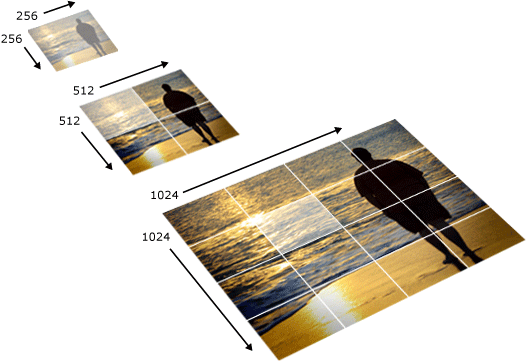
\includegraphics[scale=0.5]{img/dzi_pyramid.png}
		\caption{3 consecutive levels of a dzi image (source: https://i-msdn.sec.s-msft.com/dynimg/IC141135.png)}
		\label{fig:fig2.1}
	\end{center}
\end{figure}

The Deep Zoom Image Format (dzi)\nomenclature{dzi}{Deep Zoom Image Format} is an xml-based file format maintained by Microsoft to improve performance and quality in the handling of large image files. For this purpose an image is represented in a tiled pyramid (see fig. 2.1).

As seen in fig. 2.1 there are multiple versions of a single image in different resolutions. Each resolution in the pyramid is called a \emph{level}. At each level the image is scaled down by the factor 4 (2 in each dimension). Furthermore, the image gets tiled up into $256^2$ tiles (256 in each dimension)\cite{web:dzi}.

If a viewer wants to view a certain area of the image (e.g. the highlighted tile in the last image in fig. 2.1), only the corresponding tiles need to be loaded. This saves large amounts of bandwidth and memory. The same goes for a viewer, who is zoomed out very far. In such a view the full level of detail isn't needed, so that a version from a lower level can be loaded.

A dzi file consists of two parts: a describing .xml file\footnote{Frameworks like \emph{OpenSeaDragon} also support further formats, such as .json.} and a folder with more subfolder. Each subfolder describes a level and as such contains all the tiles for that particular level.


\section{Short Introduction to Neural Networks}
The objective of this thesis ultimately is to create training samples for NN\footnote{see chap. 1.2}. Before going into other details, it is necessary to clarify what NN are, how they work, why they need training samples and what they use them for\footnote{It should be mentioned that the scope of NN is huge and worth a whole thesis by themselves. This is nothing more than a short introduction and further consultation of literature (see e.g. \cite{Stergiou96},\cite{Egmont-Petersen02},\cite{Kriesel07},\cite{Shiffman12},\cite{Bourg04}) is highly recommended.}.

Artificial Neural Networks (NN)\nmc{NN}{Neural Networks} are a group of models inspired by Biological Neural Networks (BNN) \nmc{BNN}{Biological Neural Networks}. BNNs can be described as an interconnected web of neurons (see fig 2.x), whose purpose it is to transmit information in the form of electrical signals. A neuron receives input via dendrites and send output via axons\cite{Shiffman12}. An average human adult brain contains about $10^{11}$ neurons. Each of those receives input from about $10^4$ other neurons. If their combined input is strong enough, the receiving neuron will send an output signal to other neurons\cite{Bourg04}.

\begin{figure}[H]
	\begin{center}
		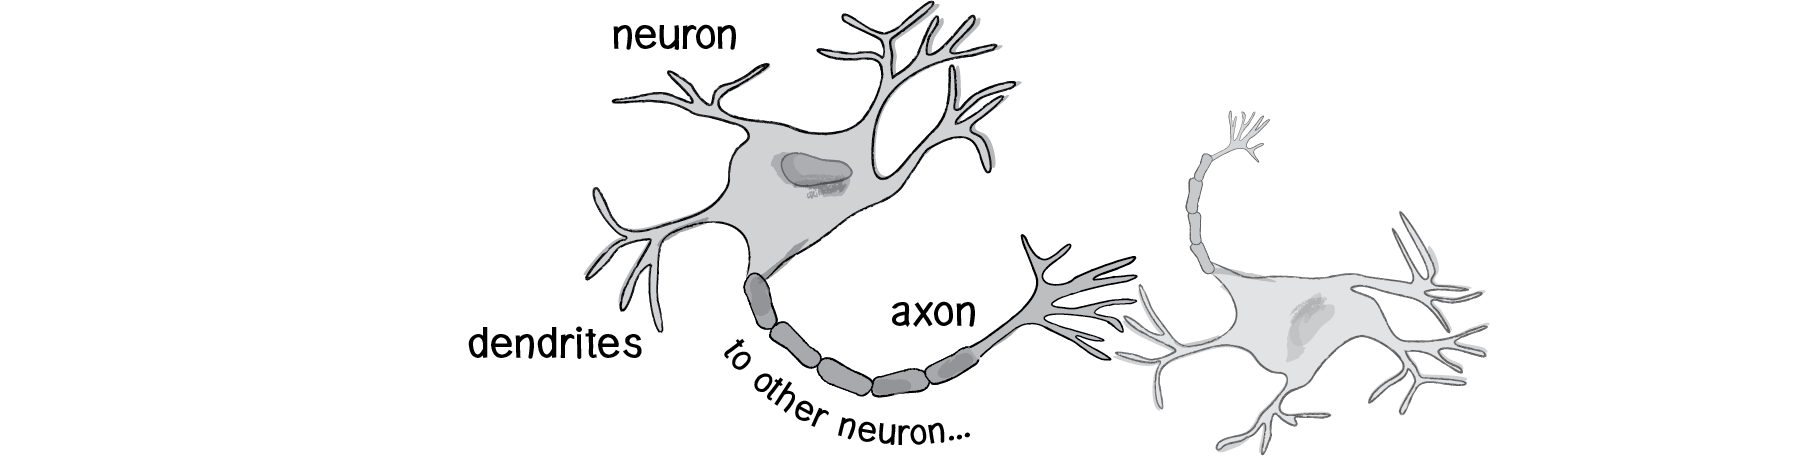
\includegraphics[scale=0.7]{img/bnn.png}
		\caption{Neuron in a BNN (source:\cite{Shiffman12})}
		\label{fig:fig2.2}
	\end{center}
\end{figure}

NN are much simpler in comparison\footnote{Usually, they don't have much more than a few dozen neurons\cite{Bourg04}.}, but generally work in the same fashion.

One of the biggest strengths of a NN, much like a BNN, is the ability to adapt by learning\footnote{As humans, NN learn by training\cite{Shiffman12}.}. This adaption is based on \emph{weights} that are assigned to the connections between single neurons. Fig 2.x shows an exemplary NN with neurons and the connections between them.

\begin{figure}[H]
	\begin{center}
		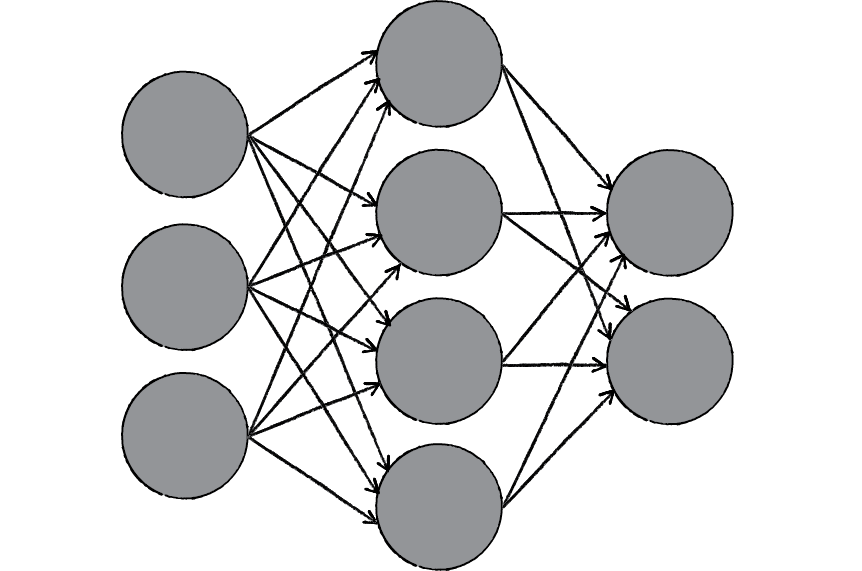
\includegraphics[scale=1.0]{img/NN.png}
		\caption{Exemplary NN (source:\cite{Shiffman12})}
		\label{fig:fig2.3}
	\end{center}
\end{figure}

Each line in fig, 2.x represents a connection between 2 neurons. Those connections are a one-directional flow of information, each assigned with a specific weight. This weight is a simple number that is multiplied with the incoming/outgoing signal and therefore weakens or enhances it. They are the defining factor of the behavior of a NN. Determining those values is the purpose of training a NN\cite{Bourg04}.

According to \cite{Shiffman12}, some of the standard use cases for NN are:

\begin{itemize}
	\item Pattern Recognition
	\item Time Series Prediction
	\item Signal Processing Perceptron
	\item Control
	\item Soft Sensors
	\item Anomaly Detection
\end{itemize}


\subsection{Methods of Learning}
There are 3 general strategies when it comes to the training of a NN\cite{Bourg04}. Those are:

\begin{enumerate}
	\item Supervised Learning
	\item Unsupervised Learning
	\item Reinforcement Learning (a variant of Unsupervised Learning\cite{Rojas96})
\end{enumerate}

\emph{Supervised Learning} is a strategy that involves a training set to which the correct output is known, as well as an observing teacher. The NN is provided with the training data and computes its output. This output is compared to the expected output and the difference is measured. According to the error made, the weights of the NN are corrected. The magnitude of the correction is determined by the used learning algorithm\cite{Rojas96}.

\emph{Unsupervised Learning} is a strategy that is required when the correct output is unknown and no teacher is available. Because of this, he NN must organize itself\cite{Shiffman12}. \cite{Rojas96} makes a distinction between 2 different classes of unsupervised learning:

\begin{itemize}
	\item reinforced learning
	\item competitive learning
\end{itemize}

Reinforced learning adjusts the weights in such a way, that desired output is reproduced. For example, a robot in a maze. If the robot can drive straight without any hindrances, it can associate this sensory input with driving straight (desired outcome). As soon as it approaches a turn, the robot will hit a wall (non-desired outcome). To prevent it from hitting the wall it must turn, therefore the weights of turning must be adjusted to the sensory input of being at a turn. Another example is \emph{Hebbian learning}\footnote{see \cite{Rojas96} for further information}\cite{Rojas96}.

In competitive learning, the single neurons compete against each other for the right to give a certain output for an associated input. Only one element in the NN is allowed to answer, so that other, competing neurons are inhibited\cite{Rojas96}.


\subsection{The Perceptron}

\subsection{Architecture of Neural Networks}


% https://www.doc.ic.ac.uk/~nd/surprise_96/journal/vol4/cs11/report.html#Introduction to neural networks

% http://natureofcode.com/book/chapter-10-neural-networks/







In a NN, regardless if artificial or biological, many neurons are interconnected with each other. The construct of interconnected neurons can be seperated into layers, of which there are three kinds:

\begin{itemize}
	\item input layer
	\item hidden layer
	\item output layer
\end{itemize}

\begin{figure}[H]
	\begin{center}
		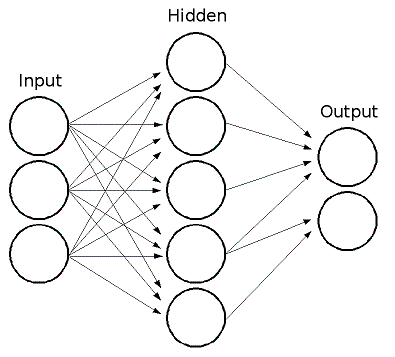
\includegraphics[scale=0.7]{img/mlp.png}
		\caption{3 layer NN (source: http://docs.opencv.org/2.4/\textunderscore images/mlp.png)}
		\label{fig:fig2.2}
	\end{center}
\end{figure}

Basically, the input layer, as the name suggests, is the layer where the NN gets its input data from. After that, there are a number of hidden layers\footnote{A NN doesn't necessarily need to have any hidden layers. For non trivial problems however, it becomes mandatory.}, which are responsible for further computation of the input values. At the end is the output layer which is responsible for communicating the results of the prior operations (compare fig. 2.2). Each single neuron has input values and an output value. Once the input reaches a certain trigger point, the cell in the neuron sends a signal as output. 

A huge benefit of NN, over other software models, is their ability to learn. While certain problems are easier to solve in a sequential, algorithmic fashion (say an equation or the towers of hanoi), certain problems are so complex that new approaches are needed, while other problems can't be solved algorithmic at all. With the use of adequate training samples, a NN can train to solve a problem, not unlike a human, by learning. Since this topic alone is enough for a number of theses, the author refers to \cite{Kriesel07} for further detailed information.


\section{Microservices}
The following section elaborates on the concept of \emph{Microservices} (MS)\nmc{MS}{Microservice}, defining what they are, listing their pros and cons, as well as explaining why this approach was chosen over a monolithic approach. A monolithic software solution is described by \cite{Lewis14} as follows:
\begin{quotation}
	"[...] a monolithic application [is] built as a single unit. Enterprise Applications are often built in three main parts: a client-side user interface (consisting of HTML pages and javascript running in a browser on the user's machine) a database (consisting of many tables inserted into a common, and usually relational, database management system), and a server-side application. The server-side application will handle HTTP requests, execute domain logic, retrieve and update data from the database, and select and populate HTML views to be sent to the browser. This server-side application is a monolith - a single logical executable. Any changes to the system involve building and deploying a new version of the server-side application."
\end{quotation}


\subsection{Definition}
MS are an interpretation of the Service Oriented Architecture. The concept is to separate one monolithic software construct into several smaller, modular pieces of software\cite{Wolff16}. As such, MS are a modularization concept. However, they differ from other such concepts, since MS are independent from each other. This is a trait, other modularization concepts usually lack\cite{Wolff16}. As a result, changes in one MS don't bring up the necessity of deploying the whole product cycle again, but just the one service. This can be achieved by turning each MS into an independent process with its own runtime\cite{Lewis14}.

This modularization creates an information barrier between different MS. Therefore, if MS need to share data or communicate with each other, light weight communication mechanisms must be established, such as a RESTful API\cite{Riggins15}.

Even though MS are more a concept than a specific architectural style, certain traits are usually shared between them\cite{Riggins15}. According to \cite{Riggins15} and \cite{Lewis14}, those are:

\begin{enumerate}[(a)]
	\item \textbf{Componentization as a Service:} bringing chosen components (e.g. external libraries) together to make a customized service
	\item \textbf{Organized Around Business Capabilities:} cross-functional teams, including the full range of skills required to achieve the MS goal
	\item \textbf{Products instead of Projects:} teams own a product over its full lifetime, not just for the remainder of a project
	\item \textbf{Smart Endpoints and Dumb Pipes:} each microservice is as decoupled as possible with its own domain logic
	\item \textbf{Decentralized Governance:} enabling developer choice to build on preferred languages for each component.
	\item \textbf{Decentralized Data Management:} having each microservice label and handle data differently
	\item \textbf{Infrastructure Automation:} including automated deployment up the pipeline
	\item \textbf{Design for Failure:} a consequence of using services as components, is that applications need to be designed so that they can tolerate the failure of single or multiple services
\end{enumerate}

Furthermore, \cite{Bugwadia15} defined 5 architectural constraints, which should help to develop a MS:

\begin{enumerate}[(1.)]
	\item \textbf{Elastic}\\
	The elasticity constraint describes the ability of a MS to scale up or down, without affecting the rest of the system. This can be realized in different ways. \cite{Bugwadia15} suggests to architect the system in such a fashion, that multiple stateless instances of each microservice can run, together with a mechanism for Service naming, registration, and discovery along with routing and load-balancing of requests.
	\item \textbf{Resilient}\\
	This constraint is referring to the before mentioned trait (h) - \emph{Design for Failure}. The failure of or an error in the execution of a MS must not impact other services in the system.
	\item \textbf{Composable}\\
	To avoid confusion, different MS in a system should have the same way of identifying, representing, and manipulating resources, describing the API schema and supported API operations.
	\item \textbf{Minimal}\\
	A MS should only perform one single business function, in which only semantically closely related components are needed.
	\item \textbf{Complete}\\
	A MS must offer a complete functionality, with minimal dependencies to other services. Without this constraint, services would be interconnected again, making it impossible to upgrade or scale individual services.
\end{enumerate}


\subsection{Advantages and Disadvantages}
% pros
One big advantage of this modularization is that each service can be written in a different programming language, using different frameworks and tools. Furthermore, each microservice can bring along its own support services and data storages. It is imperative for the concept of modularization, that each microservice has its own storage of which it is in charge of\cite{Wolff16}.

The small and focused nature of MS makes scaling, updates, general changes and the deploying process easier. Furthermore, smaller teams can work on smaller code bases, making the distribution of know how easier\cite{Riggins15}.

Another advantage is how well MS plays into the hands of agile, scrum and continuous software development processes, due to their previously discussed inherent traits.

% cons
The modularization of MS doesn't only yield advantages. Since each MS has its own, closed off data management\footnote{See 2.3.1(f) (\emph{Decentralized Data Management})}, interprocess communication becomes a necessity. This can lead to communicational overhead which has a negative impact on the overall performance of the system\cite{Wolff16}.

2.3.1(e) (\emph{Decentralized Governance}) can lead to compatibility issues, if different developer teams chose to use different technologies. Thus, more communication and social compatibility between teams is required. This can lead to an unstable system which makes the deployment of extensive workarounds necessary\cite{Riggins15}.

It often makes sense to share code inside a system to not replicate functionality which is already there and therefore increase the maintenance burden. The independent nature of MS can make that very difficult, since shared libraries must be build carefully and with the fact in mind, that different MS may use different technologies, possibly creating dependency conflicts.


\subsection{Conclusion}	
After consideration of the advantages and disadvantages of MS, the author decided in favor of using them. This is mainly due to the fact of working alone on the project, negating some of their inherent disadvantages:
\begin{itemize}
	\item Interprocess communication doesn't arise between the single stages of the process chain, since they have a set order\footnote{E.g. it wouldn't make sense trying extract a training sample without converting or annotating a WSI first.}
	\item Different technologies may be chosen for the single steps of the process chain, however, working alone on the project makes technological incompatibilities instantly visible
	\item The services shouldn't share functionality, therefore there should be no need for shared libraries
\end{itemize}
This makes the advantages outweight the disadvantages clearly:
\begin{itemize}
	\item different languages and technologies can be used for every single step of the process chain, making the choice of the most fitting tool possible
	\item WSIs take a heavy toll on memory and disk space due to their size; the use of MS allows each step of the chain to handle those issues in the most suitable way for each given step
	\item separating the steps of the process chain into multiple MS makes for a smaller and easier maintainable code base
	\item other bachelor/master students may continue to use or work on this project in the future, making the benefit of a small, easily maintainable code base twice as important
	\item the implementation of the project will happen in an iterative, continuous manner, which is easily doable with the use of MS
\end{itemize}


\section{Process Chain}
This section and its following subsections are dedicated to establish the process chain necessary to accomplish the research objectives stated in 1.2(a) - 1.2(c). The usual procedure would look as follows:

\begin{enumerate}[(1.)]
	\item convert chosen WSI $img^{wsi}_i$ to DZI format $img^{dzi}_i$
	\item open $img^{dzi}_i$ in a viewer $V$
	\item annotate $img^{dzi}_i$ in $V$
	\item persist annotations $A_i$ on $img^{dzi}_i$ in a file $f_{(A_i)}$
	\item create training sample $ts_i$ by extracting the information of $A_i$ in correspondence to $img^{dzi}_i$
\end{enumerate}

While it only makes sense to run (1.) once per $img^{wsi}_i$ to create $img^{dzi}_i$, steps (2.) - (4.) can be repeated multiple times, so that there is no need to finish the annotation of an image in one session. That makes it necessary to not only save but also load annotations. Therefore, the loading of already made annotations can be added as step (2.5). This also enables the user of editing and deleting already made annotations. Because of this, step (5.) also needs to be repeatable.

The single steps of the process chain will be sorted into semantic groups. Each group will be realized by its own MS, as stated in 2.3. The semantic groups are: conversion (1.), extraction (5.) and viewing and annotation (2. - 4.).

A MS will be introduced for each group in the following subsections(2.4.1 - 2.4.3). Those are:

\begin{itemize}
	\item \textbf{Conversion Service}\\
	This service will be responsible of the conversion from $img^{wsi}_i$ to $img^{dzi}_i$ (1.).
	\item \textbf{Annotation Service}\\
	This service will offer a GUI to view a $img^{dzi}_i$, as well as make and manage annotations (2. - 4.)
	\item \textbf{Tessellation Service}\\
	This service will be responsible for extracting a $ts_i$ from a given $A_i$ and $img^{dzi}_i$ (5.).
\end{itemize}


\subsection{Conversion Service}

The devices which create WSIs, so called \emph{whole slide scanners}, create images in various formats, depending on the producer and a lack of a defined standard\cite{Cornish13}. The Conversion Service (CS)\nmc{CS}{Conversion Service} has the goal of converting those formats to DZI\footnote{see chap. 1.2(i) and 1.2(ii) for the reasons}].

\begin{figure}[H]
	\begin{center}
		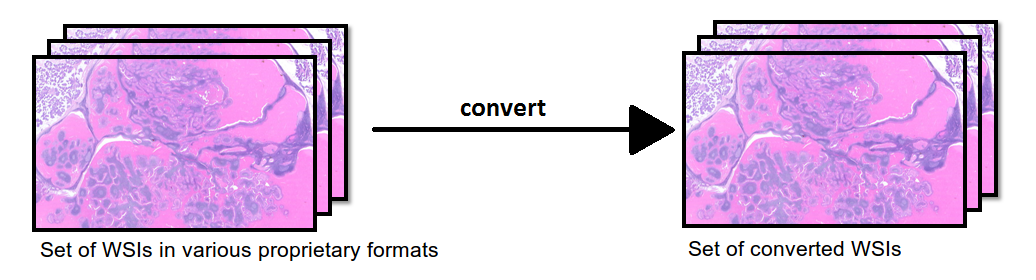
\includegraphics[scale=0.35]{img/processChainA.png}
		\caption{Visualization of the Conversion Service}
		\label{fig:fig2.1}
	\end{center}
\end{figure}

Upon invocation, the CS will take every single WSI inside a given directory and convert it to DZI. The output of each conversion will be saved in another specified folder. Valid image formats (and their corresponding producers) for conversion are:

\begin{itemize}
	\item .bif (Ventana)
	\item .mrxs (Mirax)
	\item .ndpi (Hamamatsu)
	\item .scn (Leica)
	\item .svs (Aperio)
	\item .svslide (Sakura)
	\item .tif (Aperio, Trestle, Ventana)
	\item .tiff (Philips)
	\item .vms (Hamamatsu)
	\item .vmu (Hamamatsu)
\end{itemize}


\subsection{Annotation Service}
As mentioned in 2.4, the Annotation Service (AS)\nmc{AS}{Annotation Service} will provide a graphical user interface (GUI)\nmc{GUI}{Graphical User Interface} to view a DZI, make annotations and manage those annotations. This also includes persisting made annotations in a file (see fig. 2.2).

\begin{figure}[H]
	\begin{center}
		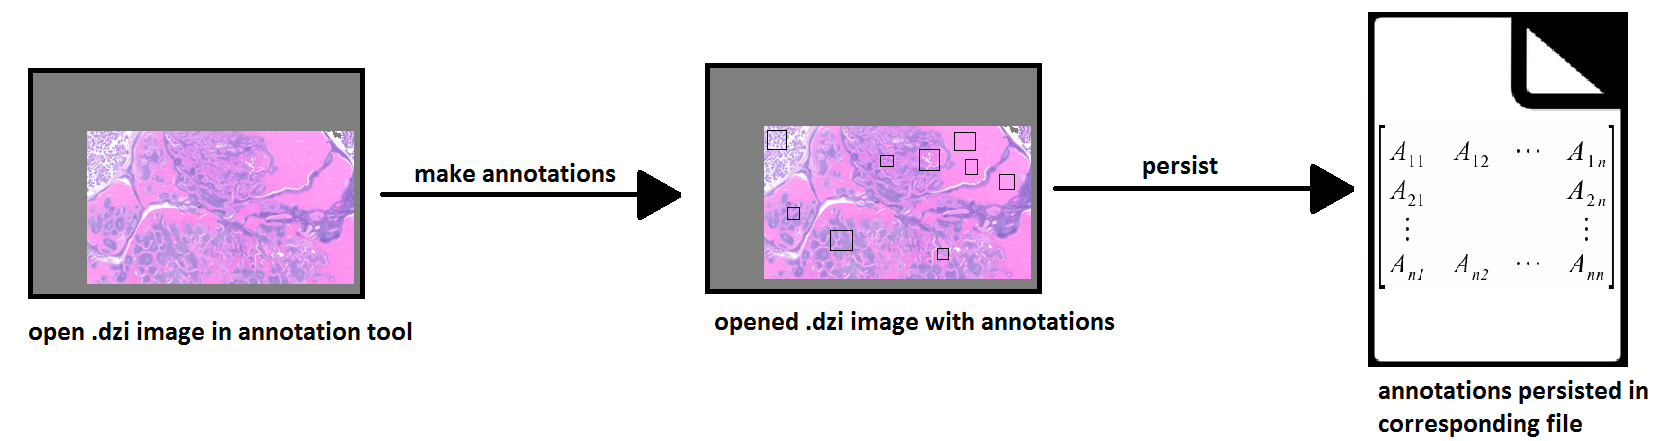
\includegraphics[scale=0.25]{img/processChainB.png}
		\caption{Visualization of the Annotation Service}
		\label{fig:fig2.4}
	\end{center}
\end{figure}

The supplied GUI will offer different tools to help the user annotate the DZI, e.g. a ruler to measure the distance between 2 points. The annotations themselves will be made via drawing a contour around an object of interest and putting a specified label to that region. To ensure uniformity of annotations, labels will not be added in free text. Instead they will be selected from a predefined dictionary.


\subsection{Tessellation Service}

The task of the Tessellation Service (TS)\nmc{TS}{Tessellation Service} is to extract annotations and their corresponding image data in such a fashion that they will become usable as training samples for NN.

\begin{figure}[H]
	\begin{center}
		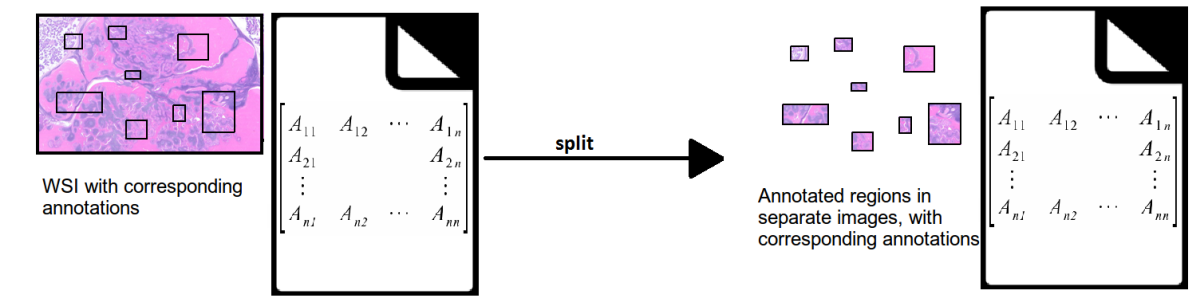
\includegraphics[scale=0.3]{img/processChainC.png}
		\caption{Visualization of the Tessellation Service}
		\label{fig:fig2.6}
	\end{center}
\end{figure}

Let there be a DZI $D$ and a corresponding set of annotations $A$. The TS will achieve the extraction by iterating over every $a_i \in A$, creating a sub-image $d_i$ which is the smallest bounding box around the region described by $a_i$ (see fig. 2.3). To be used as training sample, the TS must keep up the correspondence between $d_i$ and $a_i$.